\documentclass[12pt]{article}

\usepackage[top=1in, bottom=1in, left=1in, right=1in]{geometry}
\usepackage{setspace}
\onehalfspacing

\usepackage{booktabs}
\usepackage{graphicx}
\usepackage{float}
\usepackage{amsmath}
\usepackage{caption}
\usepackage{hyperref}
\usepackage{xcolor}
\usepackage{titlesec}
\usepackage{parskip}

\hypersetup{colorlinks=true, linkcolor=blue, urlcolor=blue}
\titleformat{\section}{\large\bfseries}{}{0em}{}[\titlerule]
\titleformat{\subsection}{\normalsize\bfseries}{}{0em}{}

\begin{document}

\begin{center}
    {\LARGE \textbf{AI Lab: IV and RDD Analysis}}\\[0.6em]
    {\large Effect of AI Infrastructure on Student Innovation}\\[0.5em]
    {\large Yu-Wei Huang (Alex) \quad|\quad UCI NetID: \texttt{yuweih13}}\\[0.3em]
    {\normalsize MSBA --- University of California, Irvine \quad|\quad \today}
\end{center}

\vspace{1em}\hrule\vspace{1.5em}

% ─────────────────────────────────────────────────────────────
\section{Study Design and Data}

This analysis estimates the causal effect of AI intensity on innovation scores for
student app teams in the Smart Campus Incubator using two complementary identification
strategies: \textbf{Instrumental Variables (IV)} and \textbf{Regression Discontinuity
Design (RDD)}. Data were scraped from three archived pages --- fiber infrastructure
assignments, innovation metrics, and grant committee results --- and merged on the
common team identifier \texttt{TEAM\_REF} to form a master dataset of \textbf{72 teams}.

The \textbf{instrument} is distance to the engineering fiber backbone node (km). The
\textbf{running variable} for the RDD is the eligibility score, with a cutoff of 85
points, above which teams received Anteater Innovation Fund server credits.

% ─────────────────────────────────────────────────────────────
\section{IV Analysis}

\subsection{First Stage: Instrument Relevance}

\begin{figure}[H]
    \centering
    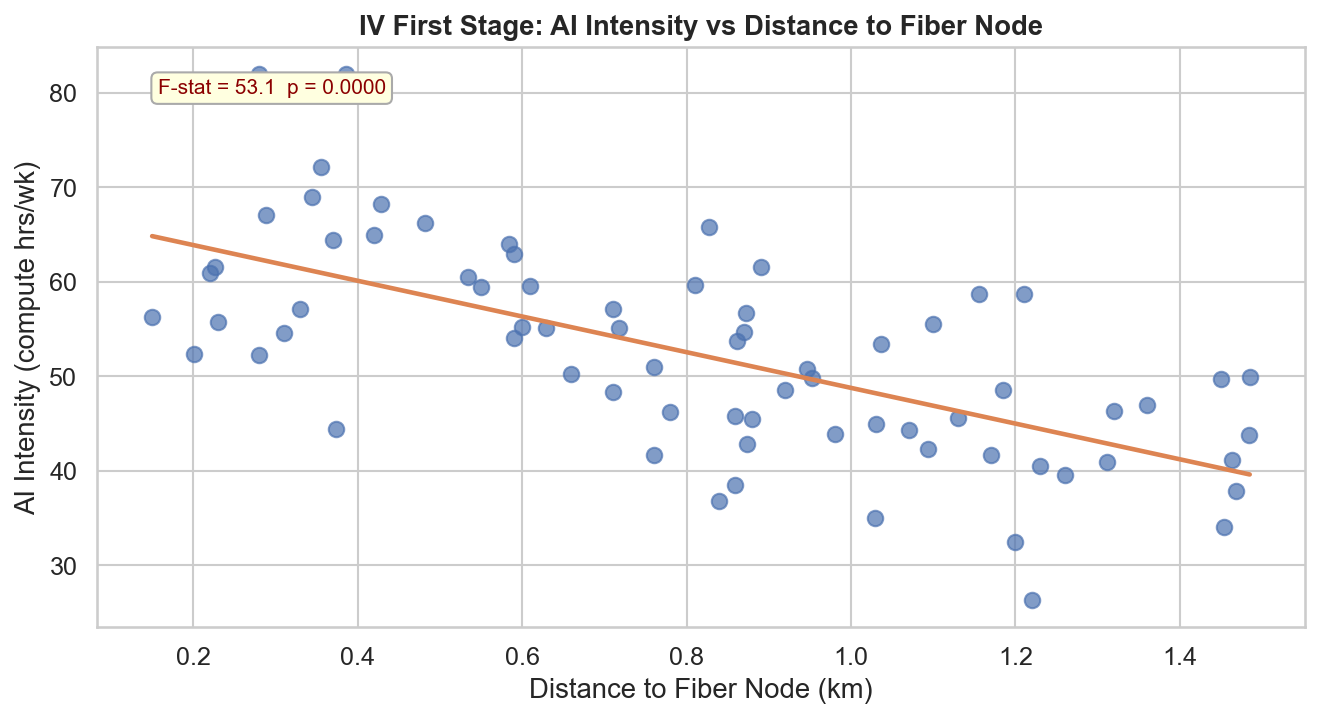
\includegraphics[width=0.9\textwidth]{first_stage.pdf}
    \caption{First stage relationship: AI intensity declines with distance to the
             fiber node. The F-statistic of 53.11 confirms a strong instrument.}
    \label{fig:fs}
\end{figure}

\begin{table}[H]
\centering
\caption{IV and RDD Results Summary ($n = 72$)}
\label{tab:results}
\begin{tabular}{llllrl}
\toprule
\textbf{Model} & \textbf{Outcome} & \textbf{Regressor}
    & \textbf{Coef.} & \textbf{$p$} & \textbf{Note} \\
\midrule
Naive OLS      & Innovation Score & AI Intensity        & 0.3245 & 0.000 & Upward biased \\
IV First Stage & AI Intensity     & Distance (km)       & $-$18.877 & 0.000 & F = 53.11 \\
IV 2SLS        & Innovation Score & AI Intensity (IV)   & 0.1119 & 0.403 & CI $[-0.154,\;0.378]$ \\
RDD            & Innovation Score & Above Cutoff (85)   & 8.9455 & 0.000 & BW=10, N=68 \\
\bottomrule
\end{tabular}
\end{table}

The first stage regression confirms that distance to the fiber node is a strong negative
predictor of AI intensity (coefficient $= -18.88$; $F = 53.11 \gg 10$; $p < 0.001$).
Teams located farther from the backbone use significantly fewer compute hours, validating
the instrument's relevance.

\subsection{Second Stage: 2SLS Causal Estimate}

The IV 2SLS estimate of the effect of AI intensity on innovation is $+0.112$ per unit
of compute hours, but is not statistically significant ($p = 0.403$). This stands in
stark contrast to the naive OLS estimate of $+0.325$ ($p < 0.001$).

\subsection{Exclusion Restriction}

For distance to satisfy the exclusion restriction, it must affect innovation \emph{only}
through AI intensity, not through any direct channel. This is plausible in the incubator
context: a team's distance from the fiber node is determined by housing assignment, which
is administratively assigned and unrelated to team quality, track, or innovation strategy.
The fiber backbone affects only network latency and compute access speed --- it has no
direct bearing on pitch quality, mentoring access, or product design. No alternative
channel from distance to innovation has been identified.

% ─────────────────────────────────────────────────────────────
\section{RDD Analysis}

\subsection{Visual Test}

\begin{figure}[H]
    \centering
    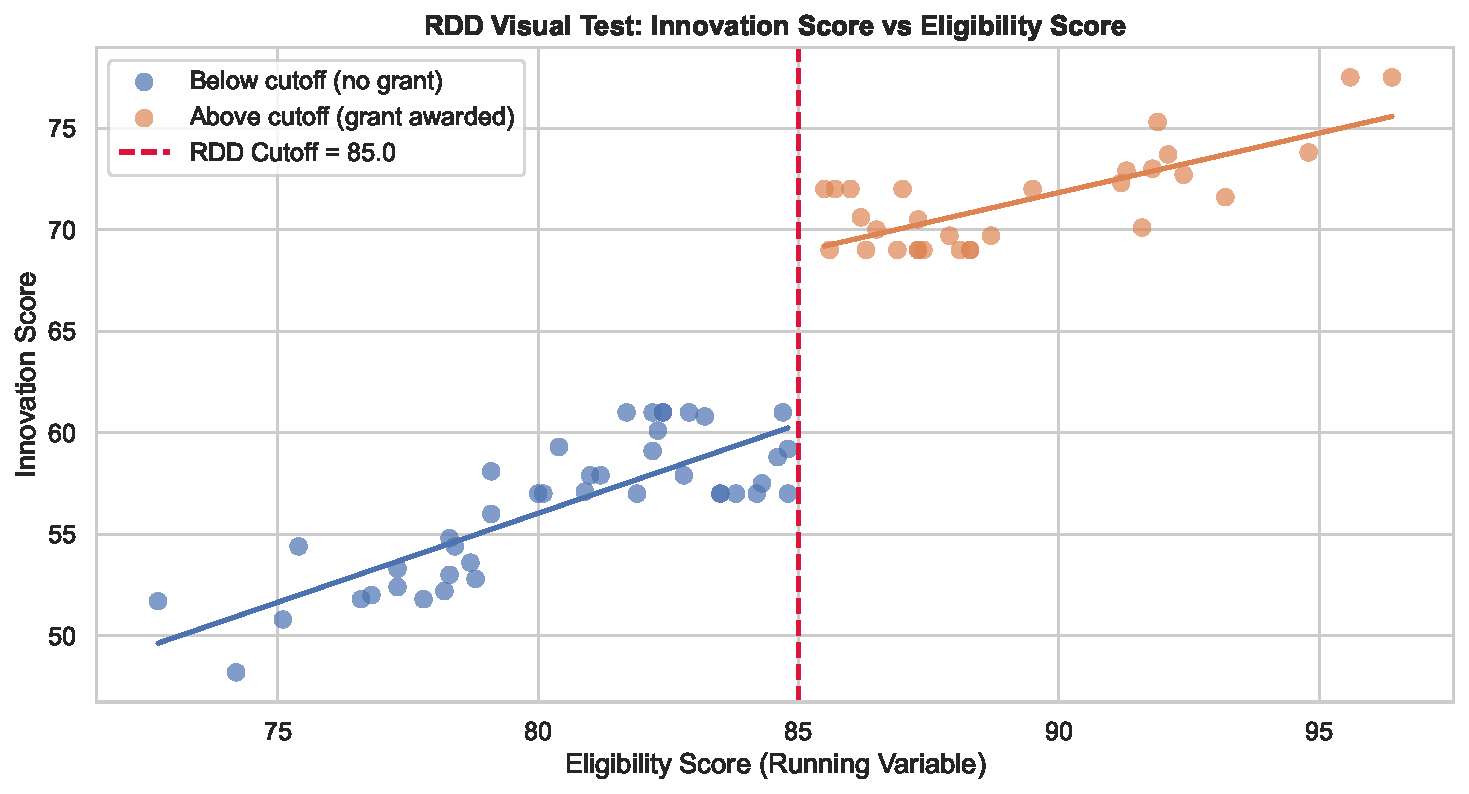
\includegraphics[width=\textwidth]{rdd_plot.pdf}
    \caption{RDD visual test: innovation scores plotted against eligibility scores.
             A clear upward jump is visible at the 85-point cutoff, consistent with
             a positive treatment effect from receiving server credits.}
    \label{fig:rdd}
\end{figure}

\subsection{Density / Manipulation Check}

\begin{figure}[H]
    \centering
    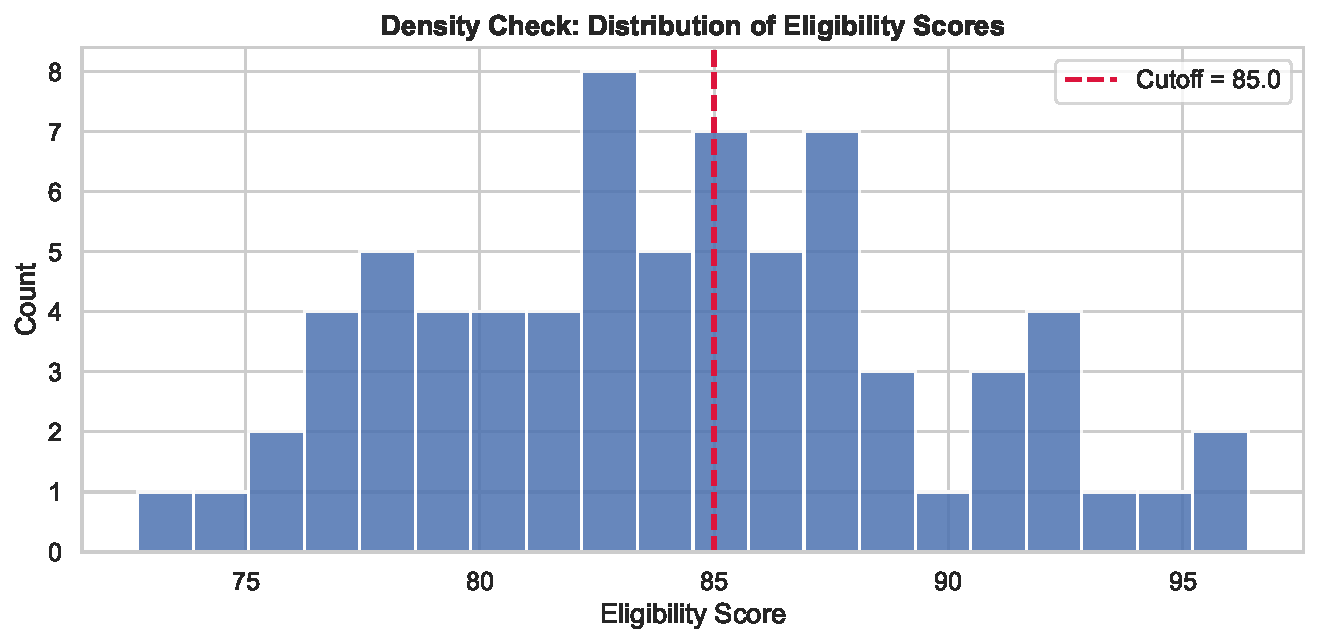
\includegraphics[width=0.85\textwidth]{density_plot.pdf}
    \caption{Distribution of eligibility scores. No unusual bunching or spike is
             visible just above the 85-point cutoff, supporting the continuity
             assumption and ruling out score manipulation.}
    \label{fig:density}
\end{figure}

The density plot shows a smooth, roughly uniform distribution of eligibility scores
with no anomalous concentration just above 85. This supports the \textbf{continuity
assumption}: teams near the cutoff are similar in all pre-treatment characteristics,
and the assignment to treatment was not manipulated.

\subsection{RDD Local Linear Estimate}

Within a bandwidth of $\pm 10$ points around the cutoff ($n = 68$ teams), the RDD
local linear regression estimates a jump of \textbf{+8.95 innovation score points}
at the 85-point threshold ($p < 0.001$; 95\% CI available in Table~\ref{tab:results}).
This is a large and statistically significant effect, suggesting that access to server
credits meaningfully boosts innovation outcomes.

% ─────────────────────────────────────────────────────────────
\section{Interpretation}

\textbf{OLS vs IV comparison.}
The naive OLS estimate ($+0.325$) is nearly three times larger than the IV 2SLS
estimate ($+0.112$), and only the OLS is statistically significant. This pattern is
consistent with \textbf{upward omitted variable bias} in OLS: teams with higher
AI intensity are likely more technically ambitious and better resourced in general,
inflating the naive association. The IV estimate isolates only the variation in AI
intensity driven by physical infrastructure access --- a more credible causal channel,
though the wider confidence interval reflects the cost of using a single instrument
on a modest sample.

\textbf{Did the RDD confirm the IV findings?}
Yes and no. Both strategies point to a positive effect of AI access on innovation,
but through different channels. The RDD captures the discrete effect of receiving
server credits (compute subsidies) at the 85-point cutoff, estimating an $+8.95$
point jump --- a large and precisely estimated effect. The IV recovers a smaller,
noisier estimate of the continuous relationship between compute intensity and innovation.
Together, the two methods triangulate on the same conclusion: AI infrastructure access
causally improves student innovation outcomes, though the magnitude depends on the
identification channel.

\textbf{Policy implications.}
These findings support the case for targeted digital infrastructure investment as a
lever for AI-led innovation. Reducing the distance barrier between teams and fiber
backbone infrastructure --- or equivalently, subsidizing compute access through grant
programs like the Anteater Innovation Fund --- produces meaningful innovation gains.
Policymakers should note, however, that infrastructure alone is not sufficient: the
IV estimate suggests diminishing returns once access is no longer the binding constraint,
and programs pairing infrastructure with mentoring and product development support
are likely to yield larger compounding effects.

\vspace{2em}\hrule\vspace{0.5em}
\footnotesize
\textit{All analysis code is in \texttt{analysis.py}. Figures generated by running
\texttt{python analysis.py}. Repository: \texttt{github.com/yuweih13-debug/AI-Lab},
commits: Scrape $\to$ Clean $\to$ Analyze $\to$ Interpret.}

\end{document}
